
%	Documentação do Trabalho Prático 1 de AEDSIII
%	@Sandro Miccoli
%
%	* Você pode identificar erros de grafia através do seguinte comando linux:
%		aspell --encoding="utf-8" -c -t=tex --lang="pt_BR" tp1.tex
%

\documentclass[12pt]{article}
\usepackage{sbc-template}
\usepackage{graphicx}
\usepackage{latexsym}
\usepackage{changepage}   % for the adjustwidth environment
\usepackage{subfigure}
\usepackage{times,amsmath,epsfig}
\usepackage{graphicx,url}
 \makeatletter
 \newif\if@restonecol
 \makeatother
 \let\algorithm\relax
 \let\endalgorithm\relax
\graphicspath{{./data/}}
\usepackage[lined,algonl,ruled]{algorithm2e}
\usepackage{multirow}
\usepackage[brazil]{babel}
\usepackage[utf8]{inputenc}
\usepackage{listings}

\usepackage{alltt}
\renewcommand{\ttdefault}{txtt}

\sloppy

\title{Programação Modular \\ Trabalho Final \\ Visualização Interativa de Agentes Inteligentes}

\author{Daniel Diniz - 2008046090 - daniel.diniz@dcc.ufmg.br\\
		Diogo Santana - 2011054308 - diogo.marques@dcc.ufmg.br\\
		Frederico Figueiredo - 2010054371 - fredfig@dcc.ufmg.br\\
		Sandro Miccoli - 2009052409 - smiccoli@dcc.ufmg.br}

\address{Departamento de Ciência da Computação -- Universidade Federal de Minas Gerais (UFMG)\\
\\
\today}


\begin{document}

\maketitle


\begin{resumo}

Esse relatório descreve como foi implementado a Visualização Interativa de Agentes Inteligentes, proposto como tema para o Trabalho Final. A Seção \ref{introducao} introduz o problema proposto e dá uma visão geral da solução implementada. Cada seção irá descrever detalhes do sistema desenvolvido, abrangendo desde o planejamento (Seção \ref{planejamento}), as decisões de implementação (Seção \ref{implementacao}) e os testes realizados (Seção \ref{testes}). Finalmente concluímos (Seção \ref{conclusao}) a documentação com reflexões sobre o aprendizado durante a execução do trabalho.

\end{resumo}

\section{Introdução}
\label{introducao}


Durante as aulas da disciplina foram vistos muitos exemplos de como implementar formas geométricas dinâmicas, então decidimos aplicar isso no nosso trabalho final. O objetivo do trabalho é unir os conceitos que aprendemos sobre programação modular e padrões de projeto e aplicá-los num contexto que seja esteticamente agradável. Isso será feito utilizando apenas formas geométricas e linhas com o intuito de gerar padrões visuais interessantes.
O modo como chegaremos nesse resultado será utilizando algoritmos de movimentação de inteligência artificial, usando conceitos como \textit{bug algorithm}, campos de potencial e desvio de obstáculos (\textit{steering}).

O planejamento inicial consiste em construir agentes inteligentes que se atraem e se repelem. Cada grupo de agentes terá uma atração a certo grupo e repulsão a outros. Por causa dessa característica de atração e repulsão, no momento em que vários agentes são atraídos por um único agente, é esperado que eles entrem em equilíbrio e formem padrões geométricos regulares.

\section{Planejamento}
\label{planejamento}

O planejamento que antecedeu à implementação ocorreu da seguinte forma: realizamos uma modelagem inicial do problema; construímos os agentes básicos; implementação do \textit{bug algorithm} com campos de potencial; implementamos o comportamento aleatório para os agentes; implementamos a interface gráfica que controla o programa e escrevemos a documentação do projeto. Além disso criamos um repositório git online para que pudéssemos trabalhar em paralelo no mesmo código e caminhar rápido com o trabalho.

\section{Implementação}
\label{implementacao}

Para a implementação dessa simulação utilizamos duas biblioteca de classes Java, \textbf{Processing} e \textbf{ControlP5}. O conjunto de
funções presentes nas classes do Processing facilitam o desenvolvimento de aplicativos orientados a arte visual e contextos gráficos em geral,
enquanto as presentes em ControlP5 nada mais que auxiliam a implementação de controladores para elementos integrados às bibliotecas do Processing. 

Foram utilizados neste sistema os padrões de projeto \textit{Singleton, Decorator e Observer}, de modo a garantir uma melhor modularização do código.
O primeiro foi utilizado para assegurar uma única instância da classe responsável pela apresentação gráfica do sistema, bem como facilitar sua
recuperação e referenciamento por outras classes do aplicativo. O mesmo padrão foi utilizado para tratar a instanciação da classe ControlP5Panel,
garantindo que quaisquer alterações feitas no painel ou qualquer informação que seja buscada por outras classes partirá de uma única instância
unificada deste, tornando-o escalável, dinamicamente modificável, estável e persistente. 

Neste painel pode se constatar, também, a aplicação do padrão \textit{Observer}. Durante a instanciação do Singleton, é criado um elemento nominado
\textit{CallbackListener}, que escuta por interações do tipo \textit{ACTION\_PRESSED} nos elementos do painel de controle, capturados apenas na instância gráfica
principal do aplicativo. Essas interações são então convertidas na forma de eventos e enviados de volta para tratamento na classe do \textbf{P5ControlPanel}.
Tudo isso a fim de garantir que as devidas funções permaneçam encapsuladas de acordo com os princípios de modularidade.

O padrão Decorator por sua vez foi implementado objetivando limitar o número de alterações necessárias na forma básica - \textit{circle} - e
permitir que novos incrementos de formas e comportamentos sejam feitos respeitando os conceitos fundamentais de Orientação a Objetos, ou seja,
grande escalabilidade com o mínimo de alteração nas classes mais abstratas e estáveis. 

A interface (Shape) representa uma forma geométrica que pode ser 'decorada' com uma infinidade de elementos diferentes. Nesse projeto
implementamos apenas diferentes tipos de círculos, tratados para todas as finalidades como comportamentos que decoram os círculos. A simulação conta com
diversas instâncias da forma \textit{circle}, que são independentemente decoradas com o devido comportamento de acordo com a interação realizada pelo usuário
através do painel de controle. Tais forças extendem a classe DecoratorShape, adicionando funcionalidade e efetivamente implementando à interface Shape.

As funcionalidades que são adicionadas às formas de Shapes são de atração e repulsão, representadas pelas classes AttractShape e RepelShape, respectivamente. Essas classes alteram o comportamento das formas em tempo de execução, permitindo que elas sejam atraídas por um único ponto e repelidas entre si. 

Esses comportamentos foram baseados em algoritmos de Interligência Artificial, como o \textit{bug algorithm}, que utilizam campos de potencial para definir o comportamento de movimentação de agentes. O campo de potencial é utilizado para definir intensidade das forças de atração e repulsão, que acaba determinando o comportamento dos agentes. É interessante destacar que o padrão Decorator pode ser aplicado várias vezes sobre os mesmos elementos, aumentando a intensidade da força calculada pelo campo de potencial.

Tudo isso é então colocado em execução sincrôna na classe Main, que sobrescreve funcionalidades implementadas na biblioteca processing para criar uma thread
que monta a simulação com as configurações iniciais e mantém todos os elementos em constante atualização e movimento.

Segue o diagrama de classes simplificado do sistema:

Após gerar o diagrama UML que indicava quais classes precisariam ser implementadas, foi definida como seria montada a estrutura de dados do programa. Abaixo, na Figura \ref{uml}, é possível ver uma versão simplificada do diagrama de classes do sistema implementado. Simplificada pois não contém nenhuma informação de atributos ou métodos, apenas de relacionamento entre as classes. 

\begin{figure}[h!]
	\centering
	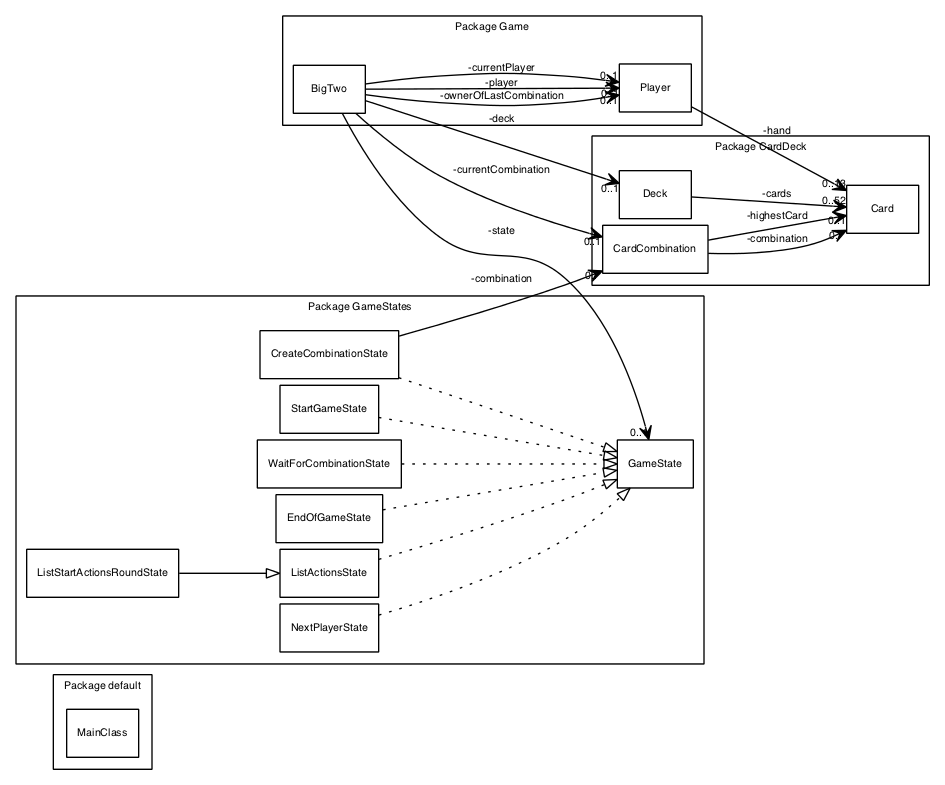
\includegraphics[width=.8\textwidth]{umlsimple.png}
	\caption{Diagrama de classes simplificado}
	\label{uml}
\end{figure}

\section{Funcionalidades}
\label{funcionalidades}
\vspace{0.4 true cm}

O programa inicia com 6 círculos em posições, direções e velocidades aleatórias, além de um ponto no centro da tela representando o centro de 
massa de atração/repulsão. Outros comportamentos podem ser adicionados a partir das seguintes teclas ou botões:

\begin{description}

\item[Botão Vectors] \hfill \\
Mostra/esconde o vetor de direção do círculo.
\vspace{0.4 true cm}

\item[Botão Connect] \hfill \\
Mostra/esconde as linhas que ligam os centros de todos os círculos.
\vspace{0.4 true cm}

\item[Botão Attract] \hfill \\
Atrai todos os círculos para o centro de massa.
\vspace{0.4 true cm}

\item[Botão Repel] \hfill \\
Aumenta a repulsão entre os círculos.
\vspace{0.4 true cm}

\item[Botão Reset] \hfill \\
Desfaz todos os comportamentos adicionados, retornando a execução ao estado inicial.
\vspace{0.4 true cm}

\item[Botão Trail] \hfill \\
Diminui a frequência de atualização do background da tela, ou seja, diminui a taxa na qual o fundo da tela é redesenhado, 
mantendo desenhos antigos na tela.
\vspace{0.4 true cm}

\item[Botão Size] \hfill \\
Aumenta/reduz o tamanho dos círculos.
\vspace{0.4 true cm}

\item[Botão RepelIntensity] \hfill \\
Aumenta/reduz a distância de repulsão entre os círculos.
\vspace{0.4 true cm}

\item[Barras horizontais] \hfill \\
Alteram a cor das linhas criadas pelo botão Connect, sendo as 3 primeiras barras referentes às cores RGB e a última referente à opacidade.
\vspace{0.4 true cm}

\item[Botão Add] \hfill \\
Adiciona um novo círculo, sendo o máximo possível igual a 30.
\vspace{0.4 true cm}

\item[Botão Remove] \hfill \\
Remove o último círculo adicionado contanto que o número de círculos na tela seja maior que 5.
\vspace{0.4 true cm}

\item[Tecla Espaço] \hfill \\
Adiciona um círculo atrator, sendo o máximo possível igual a 10. Não é afetado pelas demais funcionalidades, exceto pelo \textit{Trail}.
\vspace{0.4 true cm}

\item[Tecla Enter] \hfill \\
Adiciona um círculo repelidor, sendo o máximo possível igual a 10. Também é afetado somente pelo \textit{Trail}.
\vspace{0.4 true cm}

\item[Tecla Tab] \hfill \\
Mostra/esconde o menu de opções.
\vspace{0.4 true cm}

\item[Tecla Shift + P] \hfill \\
Tira um screenshot da tela e salva na pasta \textit{prints}

\end{description}

\section{Classes implementadas}
\label{classesimplementadas}
\vspace{0.4 true cm}
\begin{description}

\item[Main] \hfill \\
Classe principal que inicia a visualização.
\vspace{0.4 true cm}

\item[AttractShape] \hfill \\
Classe que define o comportamento de atração entre os objetos. O objeto que é decorado com essa classe atrai outros objetos de forma dinâmica.
\vspace{0.4 true cm}

\item[Circle] \hfill \\
Classe que representa o formato geométrico circular.
\vspace{0.4 true cm}

\item[DecoratedShape] \hfill \\
É uma referência para o objeto original e trabalha com uma interface para a interface Shape.
\vspace{0.4 true cm}

\item[P5ControlPanel] \hfill \\
Classe que cuida da instanciação, configuração e controlador dos eventos do programa. Possui uma interface para manipular os objetos.
\vspace{0.4 true cm}

\item[RepelShape] \hfill \\
Classe que define o comportamento de repulsão entre os objetos. O objeto que é decorado com essa classe repele outros objetos de forma dinâmica.
\vspace{0.4 true cm}

\item[Shape] \hfill \\
Interface para todos as formas de objetos.

\end{description}

\subsection{Principais métodos implementados}

Essa subseção irá listar os principais métodos implementados no sistema. Funções triviais não serão listadas, como \textit{getters}, \textit{setters} ou similares. Os métodos detalhados a seguir são os principais utilizados para a criação, decoração, controle, entre outras características.

\subsubsection{Main}

\begin{itemize}
\item \begin{large}\textit{public void setup()}\end{large}\\	
\subitem \textbf{Descrição:} Certifica de que somente uma instância do painel de controle existe.
\end{itemize}

\vspace{0.2 true cm}

\begin{itemize}
\item \begin{large}\textit{public void reset()}\end{large}\\
\subitem \textbf{Descrição:} Redefine todas as formas para o formato inicial.
\end{itemize}

\vspace{0.2 true cm}

\begin{itemize}
\item \begin{large}\textit{public synchronized void draw()}\end{large}\\
\subitem \textbf{Descrição:} Responsável pelo redesenho do formato de cada círculo.
\end{itemize}

\vspace{0.2 true cm}

\begin{itemize}
\item \begin{large}\textit{private void connectShapes()}\end{large}\\
\subitem \textbf{Descrição:} Desenha as linhas entre cada círculo.
\end{itemize}

\vspace{0.2 true cm}

\begin{itemize}
\item \begin{large}\textit{public synchronized void keyPressed(KeyEvent e)}\end{large}\\
\subitem \textbf{Descrição:} Realiza a escuta para o tratamento das teclas espaço e enter, além de lidar com a criação da atração ou repulsão dos objetos.\subitem \textbf{Parâmetros:} Recebe uma tecla de evento.
\end{itemize}

\vspace{0.2 true cm}

\subsubsection{AttractShape}

\begin{itemize}
\item \begin{large}\textit{private void attractOtherShapes()}\end{large}\\
\subitem \textbf{Descrição:} Realiza o envio da localização de cada elemento para lidar com as colisões na repulsão.
\end{itemize}

\vspace{0.2 true cm}

\begin{itemize}
\item \begin{large}\textit{public void forces(Shape targetLoc)}\end{large}\\	
\subitem \textbf{Descrição:} Essa função aumenta ou diminui a intensidade da repulsão entre os elementos.
\subitem \textbf{Parâmetro:} Recebe como parâmetro o tipo Shape, que é o formato dos objetos.
\end{itemize}

\vspace{0.2 true cm}

\subsubsection{Circle}

\begin{itemize}
\item \begin{large}\textit{public void display()}\end{large}\\
\subitem \textbf{Descrição:} Desenha na tela o círculo.
\end{itemize}

\vspace{0.2 true cm}

\begin{itemize}
\item \begin{large}\textit{public void drawVectors()}\end{large}\\
\subitem \textbf{Descrição:} Desenha o vetor que mostra a direção do movimento dos objetos.
\end{itemize}

\vspace{0.2 true cm}

\begin{itemize}
\item \begin{large}\textit{public void move()}\end{large}\\
\subitem \textbf{Descrição:} Movimenta os elementos na tela.
\end{itemize}

\vspace{0.2 true cm}

\begin{itemize}
\item \begin{large}\textit{public void bounds()}\end{large}\\
\subitem \textbf{Descrição:} Certifica que os objetos fiquem dentro dos limites da tela.
\end{itemize}

\vspace{0.2 true cm}

\subsubsection{P5ControlPanel}

\begin{itemize}
\item \begin{large}\textit{public static P5ControlPanel getInstance(PApplet source)}\end{large}\\
\subitem \textbf{Descrição:} Certifica de que somente uma instância do painel de controle existe.Realiza o controle da criação de uma combinação para ser jogada.
\subitem \textbf{Parâmetro:} Recebe como parâmetro o PApplet, que é uma subclasse do java que controla o painel.
\end{itemize}

\vspace{0.2 true cm}

\subsubsection{RepelShape}

\begin{itemize}
\item \begin{large}\textit{public void forces(Shape targetLoc)}\end{large}\\
\subitem \textbf{Descrição:} Essa função aumenta ou diminui a intensidade da repulsão entre os elementos.
\subitem \textbf{Parâmetro:} Recebe como parâmetro o tipo Shape, que é o formato dos objetos.
\end{itemize}

\vspace{0.2 true cm}

\section{Testes}
\label{testes}
O desenvolvimento deste aplicativo passou por diversas fases até chegar ao estado de arte em que se encontra. Por se tratar também de um conceito que pode ser considerado bastante abstrato por alguns, não havia, inicialmente, uma ideia fixa de como seria o estado final do programa. Assim, seguem algumas imagens das primeiras versões e ideias que tivemos, que podem ser consideradas também como testes para descobrirmos os potenciais que poderiamos atingir, além de servir como motivação para a evolução incremental da ideia.

\begin{figure}[h!]
	\centering
	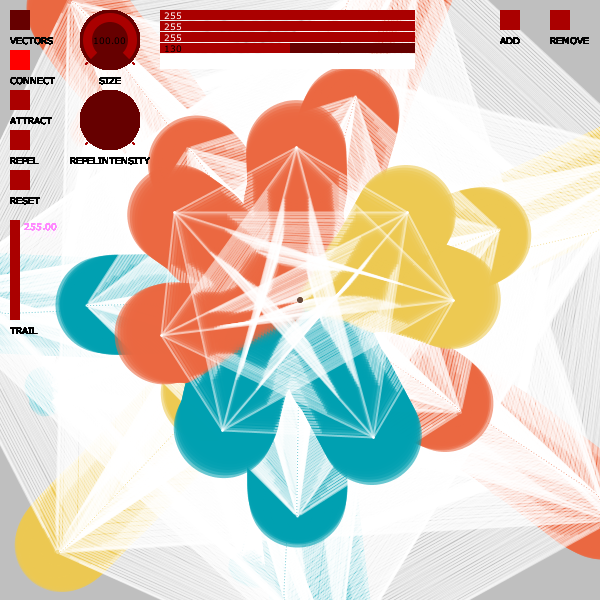
\includegraphics[width=.8\textwidth]{teste1.png}
	\caption{Visualização de Teste 1}
	\label{umlfull}
\end{figure}

\begin{figure}[h!]
	\centering
	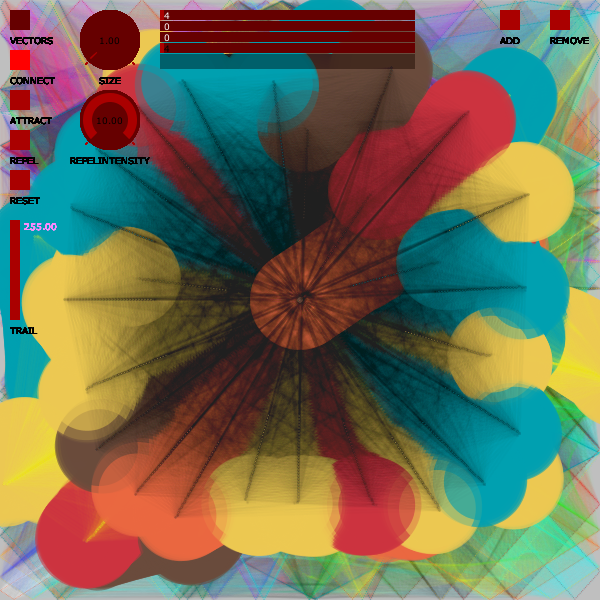
\includegraphics[width=.8\textwidth]{teste2.png}
	\caption{Visualização de Teste 2}
	\label{umlfull}
\end{figure}

\section{Conclusão}
\label{conclusao}

A partir deste trabalho foi possível aprimorar nossos conhecimentos em programação modular pela aplicação de conceitos como padrões de projeto, interface gráfica, herança, polimorfismo e encapsulamento de dados. Além do mais, o projeto também proporcionou uma experiência de desenvolvimento em equipe e da modelagem em conjunto de um problema, aproximando-nos à realidade de desenvolvimento do mercado.

Foi interessante visualizar como padrões de projeto podem alterar o comportamento do programa criado, especialmente no caso de uma aplicação gráfica. No caso do padrão Decorator, podemos ver ele sendo adicionado várias vezes sobre o mesmo elemento e aumentando a atração e repulsão entre os elementos.

Apesar das dificuldades de implementação do comportamento dos agentes, os resultados mostraram-se satisfatórios e até mesmo melhores do que o esperado. Gerar padrões de imagens mostrou-se bastante divertido e foram gastas horas apenas experimentando as diversas combinações de funcionalidades. \cite{github}

\bibliographystyle{sbc}
\bibliography{tp1}

%\begin{figure}[h!]
%	\centering
%	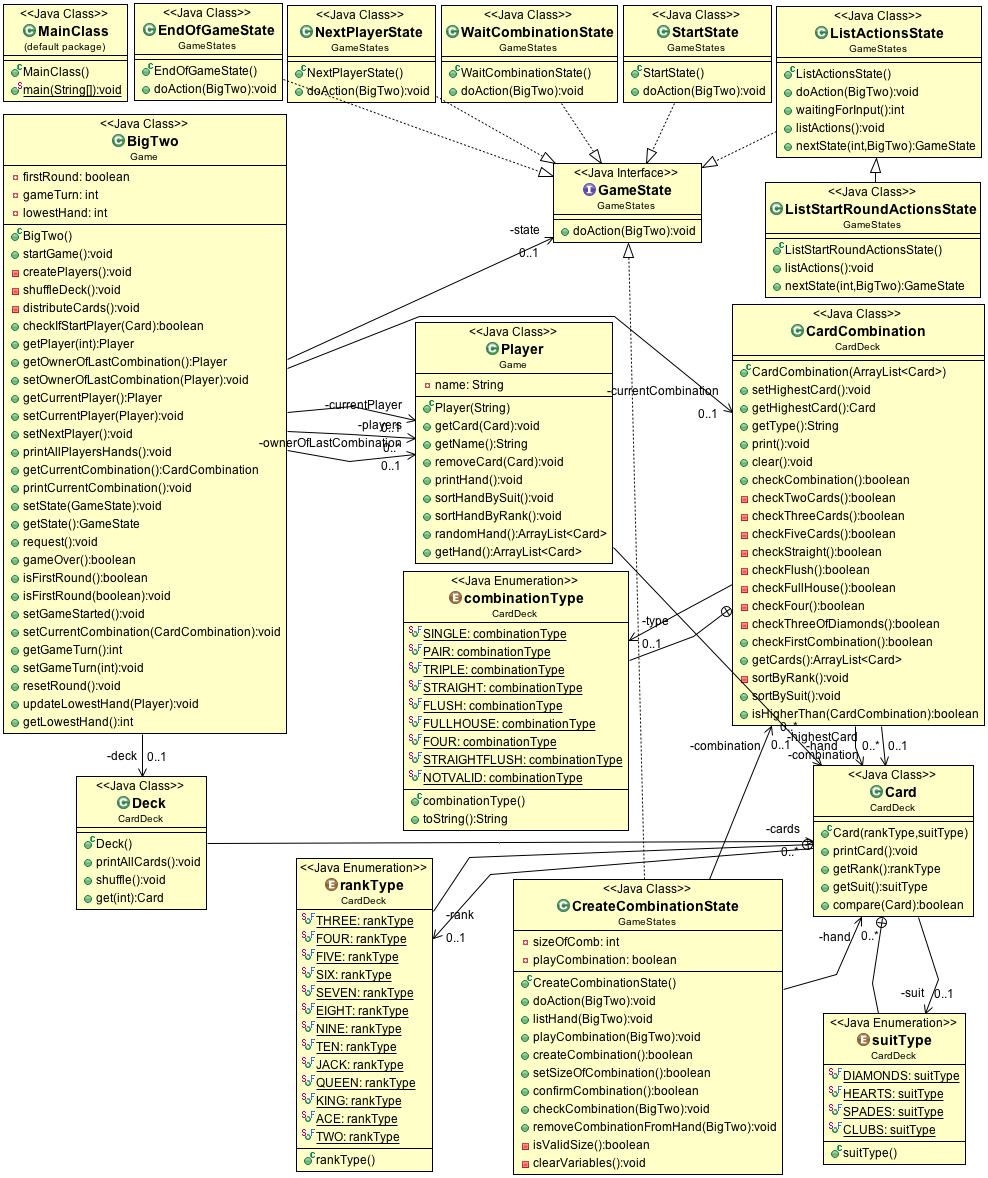
\includegraphics[width=.8\textwidth]{umlfull.png}
%	\caption{Diagrama de classes completo}
%	\label{umlfull}
%\end{figure}

\end{document}
